\usetikzlibrary{patterns}

\newsavebox{\decryptGenCode}
\begin{lrbox}{\decryptGenCode}
\begin{lstlisting}
int KEY = RAND();
write(MOV_OPCODE, ...);
...
for (int i = RAND(); i > 0; --i) 
    write(NOP_OPCODE);
...
write(XOR_OPCODE, KEY, ...);
...
\end{lstlisting}
\end{lrbox}

\begin{frame}[fragile,label=olig]{oligomorphic virus/worm}
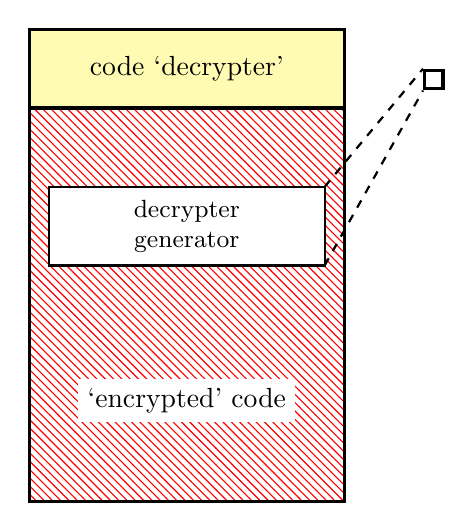
\begin{tikzpicture}
\draw[fill=yellow!30,very thick] (0, 0) rectangle ++(4, -1) node[midway] {code `decrypter'};
\draw[pattern=north west lines,pattern color=red,very thick] (0, -1) rectangle ++(4, -5);
    \node[anchor=south,fill=white] at (2, -5) {`encrypted' code};
    \draw[fill=white,thick,font=\small] (0.25, -2) rectangle ++ (3.5, -1) node[midway,align=center] {
        decrypter \\
        generator
    };
\node[anchor=north west,draw,very thick,font=\small] (decrypt gen code) at (5, -0.5) {
\usebox{\decryptGenCode}
};
\draw[thick,dashed] (3.75, -2) -- (decrypt gen code.north west);
\draw[thick,dashed] (3.75, -3) -- (decrypt gen code.south west);
\end{tikzpicture}
\end{frame}

\begin{frame}{producing changing malware}
    \begin{itemize}
    \item `encrypted' code can generate new decrypter
    \item not just {\tt nop}:
    \vspace{.5cm}
    \item switch between synonym instructions
        \begin{itemize}
        \item \texttt{add \$4, ...}, \texttt{sub \$-4, ...}
        \end{itemize}
    \item swap registers
    \item random instructions that manipulate `unused' registers
    \item \ldots
    \item template to generate a bunch of decrypters
        \begin{itemize}
        \item Szor calls such malware ``oligomorphic''
        \end{itemize}
    \end{itemize}
\end{frame}

